%!TEX root = ../../super_main.tex

\chapter{Architecture}
\label{cha:architecture}

This chapter introduces the architecture that will facilitate a solution corresponding to the vision in \secref{sec:vision}. An overview of the architecture is shown in \figref{fig:system_architecture}, where it can be seen that we have two main components, a server and a client. A description of the components, their overall purpose, the communication between them, and their subcomponents is covered in this chapter. More detailed descriptions of the features they provide are covered in the following chapters: \charef{cha:security}, \charef{cha:gathering_sensor_data}, and \charef{cha:user_interfaces}. 

\begin{figure}[!htbp]
    \centering
    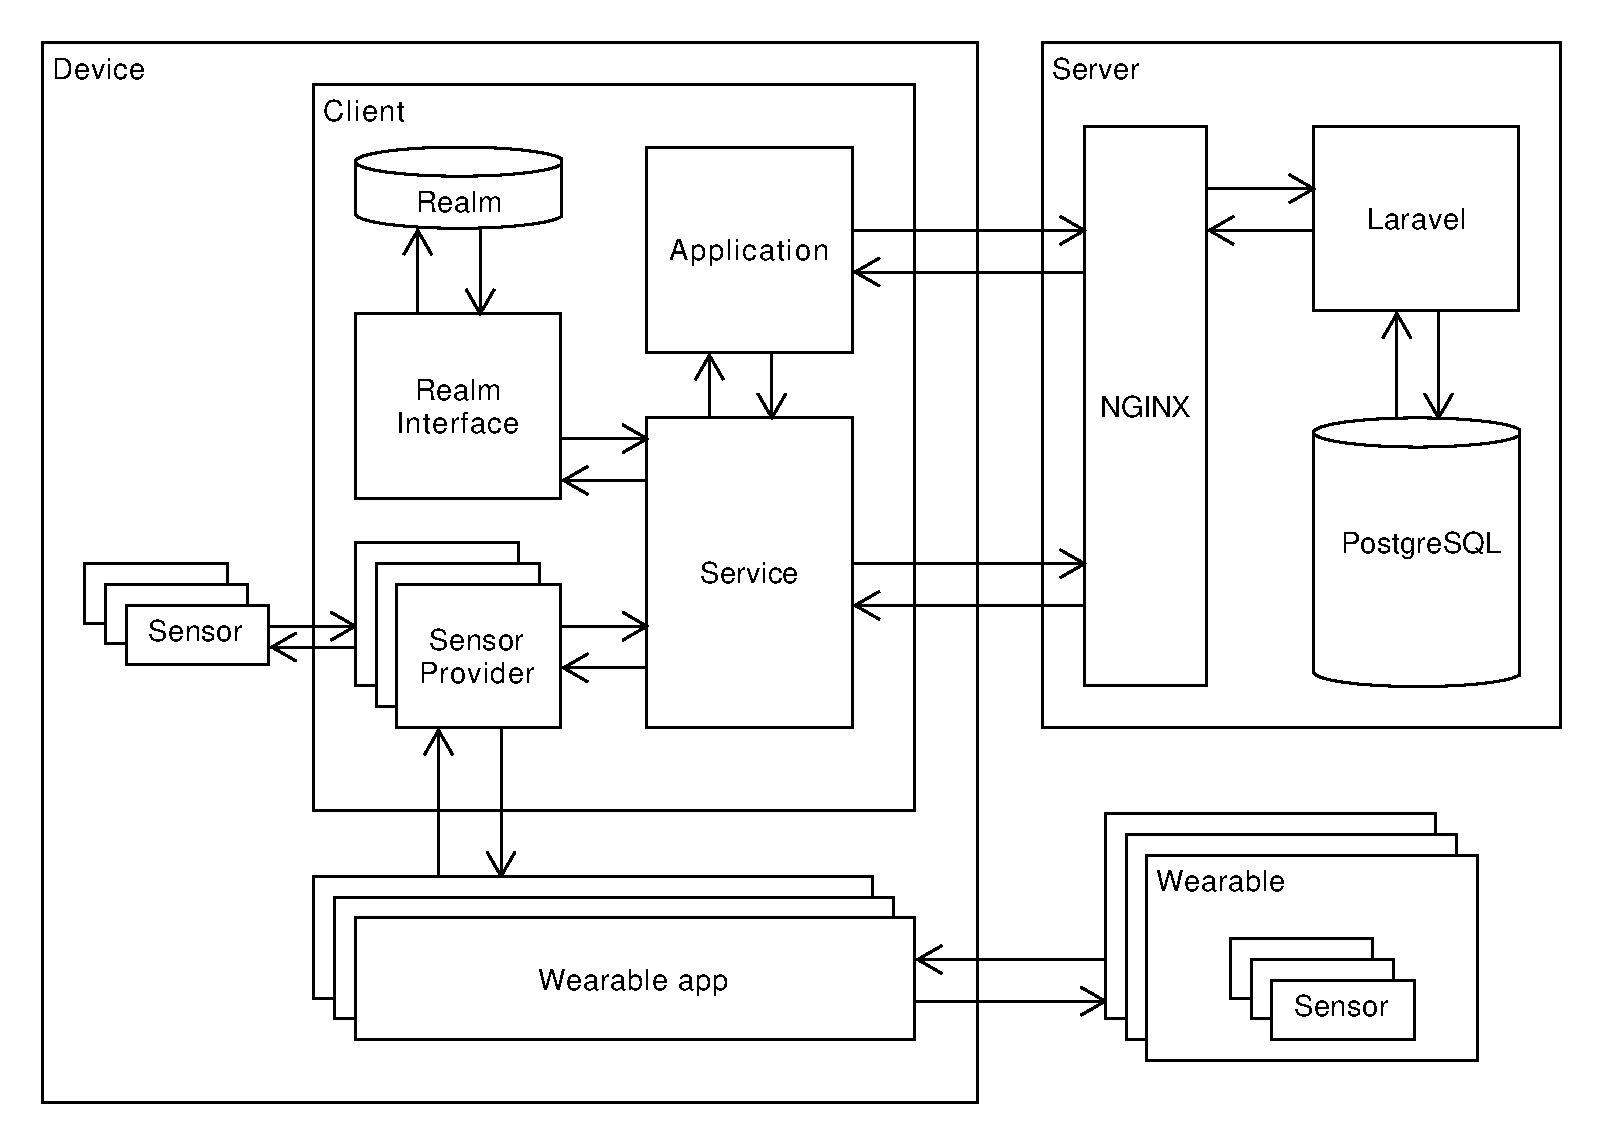
\includegraphics[width=\textwidth]{graphic/architecture/architecture.pdf}
    \caption{An abstract overview of the overall system architecture.}
    \label{fig:system_architecture}
\end{figure}
\FloatBarrier

%!TEX root = ../../super_main.tex
\section{Server}
The server provides the interface for the customers of the system, the ones in need of campaigns. Besides allowing the customers to specify campaigns the, server is also responsible for handling the upstream of snapshots from the devices of the participants. Meaning that the server has both a application programming interface (API) \todo{check if this is the first place we mention API} and a graphical user interface (GUI) \todo{check if this is the first place we mention GUI} for the customers. The server runs a web server technology called NGINX which handles the network communication using the hyper text transfer protocol (HTTP) \todo{check if this is the first place we mention HTTP} and allows for using transport layer security (TLS) \todo{check if this is the first place we mention TLS}. Furthermore this web server is also able to communicate with the underlying operating system to be able to read files from disk and interpret PHP code.
\\\\
With these features of NGINX the server is now able to facilitate the web framework Laravel. This framework builds on the model-view-controller (MVC) pattern. This allows us to route incoming requests and handle them as both application request but also as user requests. 

\todo[inline]{Snak om PostgreSQL}

%!TEX root = ../../super_main.tex

\section{Client Application}
\label{sec:client_application}

The device component is the part of the system that should run directly on the smartphone of the participant. This component is responsible for interacting with the participants, gather data from the sensors on the device, and communicating with the other devices in order to get data from wearables. The sensors represent the underlying hardware, and the Wearable Application is the interface from the client application to external wearable sensors, which in our case is the Microsoft Health application that communicates with Microsoft Band 2 we have implemented support for in the system.
\\\\
The smartphone application contains a service component that is the main controller of the client application. This service runs independently in the background at all times, and is the part of the system on a device that communicates with the different sensor providers, and also uploads the collected snapshots to the server. Furthermore it is also responsible for prompting the participants to answer the questionnaires. This service is completely detached from the graphical interface and it runs in its own seperate process, since it needs to be responsive to changes read by sensors and in other data sources. This seperation is furthermore beneficial, because it allows the Android OS to properly close and free the UI components when they are not used and deallocate all memory used by them. 
\\\\
The UI components consists of two interfaces, a settings interface and a questionnaire interface. The settings interface allows for the participant to browse details and join campaigns. Furthermore, it also has some communication with the web server where it fetches the specifications of campaigns, and reports back to the server which campaigns the participants has joined. The questionnaire interface is a series of user inputs where the participants can provide answers for the questions of a questionnaire. This interface is prompted to the user by using notifications, which are sent by the service for every snapshot, in order to obtain labels on the data if possible.
\\\\
The service component is also in need of some persistent storage on the device, to ensure that it can store gathered snapshots, so that it can upload the data using best practices in regards of power consumption and robustness as described in \secref{sec:general_strategies}. For this reason the application has a storage module where we utilize a library called \mono{realm}, which will be further describe in \secref{sub:local_storage}.
\\\\
Lastly the service component is heavily dependent on the sensor providers, which are providers that abstracts various types of sensors, for example hardware sensors on the device, software sensors, and external sensors from wearable and so on. From the service point of view, it only needs to manage the specification of campaigns and request the data from these providers accordingly before it stores the data that has been gathered from these providers on the device. The controller of the service assumes that the interface of these providers guarantees the amount of data requested and that they keep their deadlines in regards to timing of measurements.

%!TEX root = ../../../super_main.tex
\subsection{Client Requests}
\label{sub:client_requests}
The Android client needs to be able to access these routes somehow and retrieve the information they need to know to send the correct data back to the server as snapshots. There are a few different situations where such a interaction between the client should take place, some will be GUI related and some concerned about retrieving necessary data for the application to do the data gathering. Even though the communication occurs with different purposes most of the aspects of communicating over HTTP, such as establishing a connection and encoding its messages, can be generalized to a common class structure. To simplify the process of these issues we chose to utilize a library, called Webb\footnote{https://github.com/hgoebl/DavidWebb}, handling all the HTTP communication and encoding through a simple interface. Even though we use this library there are still some aspects that can be further generalized, namely ensuring that the communication happens asynchronously and thereby not blocks the applications main thread, ensuring that the right headers and request type is sent, and lastly make some modifications to the TLS verification (see \secref{sec:transport_layer_security}). The way we generalized these aspects were by extending (inheriting from) a class in the Android framework called \mono{AsyncTask}, which is an abstract class with an abstract method, named \mono{doInBackground}. This is the primary method of the \mono{AsyncTask} and is the one method that is executed in a background thread. Besides the abstract method the class also contains different empty overridable methods that will be called during the tasks life cycle, such as \mono{onPreExecute}, which will be called prior to the execution of the task and \mono{onPostExecute}, which as the name indicates will be called after the execution of the task. Both of these methods will be run on the main thread, which allows them to modify for example GUI elements. We found that, in generalizing the communication with the server, we needed to ensure that the response code matches what we expected in the different situations, such as 200 (status OK), and would otherwise need to make some error handling. We also figured that we often would need to specify what to happen if there were no available connection to the server, such that there were no response code returned. Therefore we overrode the \mono{onPostExecute} method as seen in \lstref{lst:on_post_execute}. 

\lstinputlisting[
   style = Java,
   caption = {The \mono{onPostExecute} method, which is called after the asynchronous task has completed.},
   label = {lst:on_post_execute},
   float=!htbp,
]{content/architecture/code_snippets/onPostExecute.java}
\FloatBarrier

Here we firstly check if the response parameter is null, in which case something went wrong in establishing the connection to the server, and the abstract method \mono{onConnectionFailure} will be called. Otherwise we check if the response code matches what we expect, and if it is we call the abstract method \mono{onResponse\-Code\-Matching} and if it does not we call \mono{onResponseCodeNotMatching}. These methods can then be overridden in an anonymous class or a normal class. The response code from the snippet is set through the constructor of the method, along with the the URL the request should be sent to and the request method. The response that the \mono{onPostExecute} in \lstref{lst:on_post_execute} receives as an argument is the result of the doInBackground process, which can be seen in \lstref{lst:do_in_background}. 

\lstinputlisting[
   style = Java,
   caption = {The actual task being executed on a background thread.},
   label = {lst:do_in_background},
   float=!htbp,
]{content/architecture/code_snippets/doInBackground.java}
\FloatBarrier

In this method we firstly create a custom \mono{TrustManager} and \mono{HostnameVerifier}, which is connected to the Transport Layer Security that we utilize and will be described in \secref{sec:transport_layer_security}. This is followed by setting some of the properties that we want to apply to every request, such as adding the ``X-requested-with''-header describing that the request is an Ajax request and not a normal web page request. This is followed by a check of which method is requested in the constructor and use the Webb library to create a request of that type, and use it as a parameter for the abstract method called sendRequest. As with the other abstract methods the \mono{sendRequest} method can be overridden to specify different aspects of the request, such as what the parameters for the request should be as well as how many reties there should be.
